\documentclass[14pt]{extarticle}

\usepackage{extsizes}
\usepackage{graphicx}
\usepackage[utf8]{inputenc}
\usepackage[russian]{babel}
\usepackage{indentfirst}
\usepackage{multirow}
\usepackage{subcaption}
\usepackage[normalem]{ulem}

\usepackage{lipsum}
\newenvironment{bottompar}{\par\vspace*{\fill}}{\clearpage}

\usepackage{color}
\usepackage{hyperref}
\hypersetup{
    colorlinks=true, %set true if you want colored links
    linktoc=all,     %set to all if you want both sections and subsections linked
    linkcolor=blue,
}

\newcommand{\cmmnt}[1]{\ignorespaces}

\newcounter{question}

\newcommand\Que[1]{%
    \begin{minipage}{\textwidth}
    \leavevmode\par
    \stepcounter{question}
    \noindent
    {\large\textbf{\thequestion. #1}}\par}

\newcommand\Ans[2][]{%
    \leavevmode\par\noindent
    {\leftskip37pt
    \textbf{#1}#2\par}
    \end{minipage}}

\newcommand\Partans[2][]{%
    \leavevmode\par\noindent
    {\leftskip37pt
    \textbf{#1}#2\par}}

\usepackage{fancyhdr}

\pagestyle{fancy}
\fancyhf{}
\rhead{\thepage}
\lhead{Памятка первокурсника}

\begin{document}
\begin{titlepage}

\center % Center everything on the page

%----------------------------------------------------------------------------------------
%   HEADING SECTIONS
%----------------------------------------------------------------------------------------

\textsc{\Large Совет студентов}\\ % Name of your university/college
\textsc{\Large Факультета Радиотехники и Кибернетики}\\[3cm] % Name of your university/college

%----------------------------------------------------------------------------------------
%   LOGO SECTION
%----------------------------------------------------------------------------------------

\begin{center}
    
\includegraphics[width = 130 mm]{resources/logo.png}
    \\[2cm]
\end{center}

%----------------------------------------------------------------------------------------
%   TITLE SECTION
%----------------------------------------------------------------------------------------


    { \huge \bfseries ПАМЯТКА }\\[0.5cm]
    { \huge \bfseries ПЕРВОКУРСНИКА}

\begin{bottompar}
    {\Large Долгопрудный 2018г.}
\end{bottompar}
\vfill % Fill the rest of the page with whitespace

\end{titlepage}

\tableofcontents

%%%%%%%%%%%%%%%%%%%%%%%%%%%%%%%%%%%%%%%%%%%%%%%%%%%%%%%%%%%%%%
\clearpage
\section{Введение}
\parДанная памятка является квинтэссенцией многолетнего опыта студентов ФРТК.
Для облегчения вашего периода адаптации на Физтехе мы собрали большинство
часто задаваемых вопросов и ответов на них в данном материале. Предлагаем
вам полностью прочитать раздел с вопросами (лучше всего — подряд). В конце
памятки размещены полезные справочные материалы.

Если у вас появятся замечания или предложения по содержимому памятки, вы
можете прислать их \href{https://vk.com/philalala}{Филиппу Микояну} или по адресу \underline{\textbf{philippe.mikoyan@frtk.ru}}.

И не забудьте вступить в \href{https://vk.com/drec_81x}{группу 1-го курса}!
\begin{bottompar}

Памятка подготовлена коллективом Совета студентов ФРТК МФТИ.
Текст распространяется по лицензии CC-BY-NC.
\\ \\
Общая редакция и содержание: Андрей Гущин, Данил Калабин, Максим Кузнецов.
\\
Затехано и отредактировано в 2017 и 2018 годах Микояном Филиппом.
\\ \\
    \textit{Благодарим за ценные замечания Дмитрия Девятилова, Александра Куриловича, Евгения Майорова, Павла Кукушкина, Рустема Фейзханова, Леонида Шепурёва и Якова Львовича.}

\end{bottompar}
%%%%%%%%%%%%%%%%%%%%%%%%%%%%%%%%%%%%%%%%%%%%%%%%%%%%%%%%%%%%%%
\clearpage
\section{Контакты}
\subsection{Директорат ФРКТ}
\begin{figure}[h!]
\captionsetup[subfigure]{labelformat=empty,justification=centering,textfont=normalfont}
\captionsetup{labelformat=empty,justification=centering,textfont=normalfont}
    \begin{subfigure}[b]{0.5\linewidth}
        \centering
        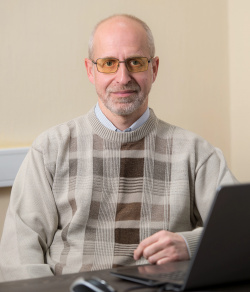
\includegraphics[width=0.65\linewidth]{resources/dvork.jpg}
        \caption{Дворкович Александр Викторович \\ \textbf{Директор ФРКТ}}
    \end{subfigure}
    \begin{subfigure}[b]{0.5\linewidth}
        \centering
        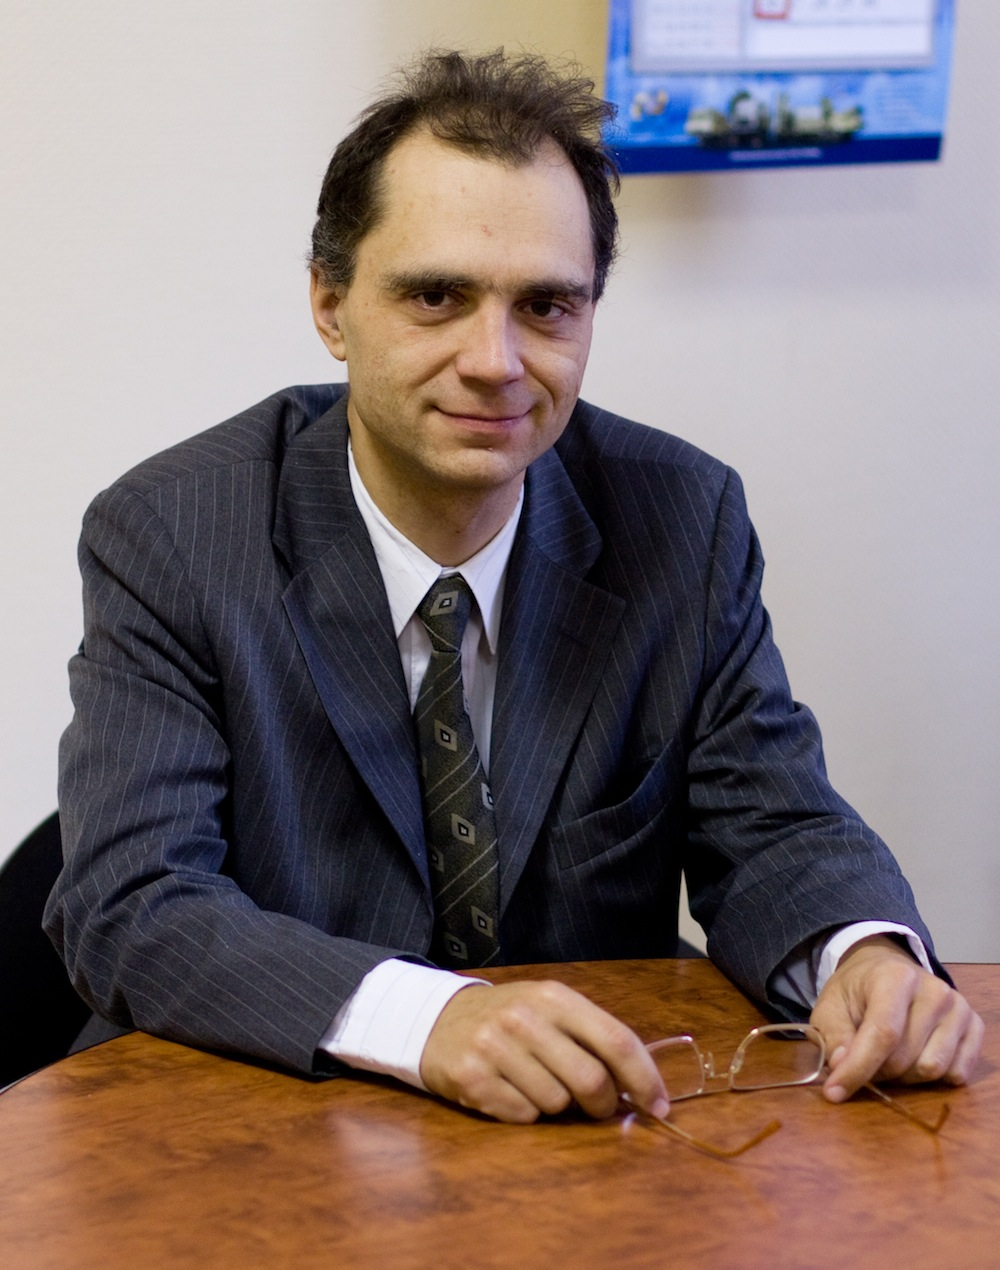
\includegraphics[width=0.65\linewidth]{resources/russk.jpg}
        \caption{Русскин Сергей Олегович \\ \textbf{Зам. дир. по уч.-метод. работе}}
    \end{subfigure}
    \begin{subfigure}[b]{0.32\linewidth}
        \centering
        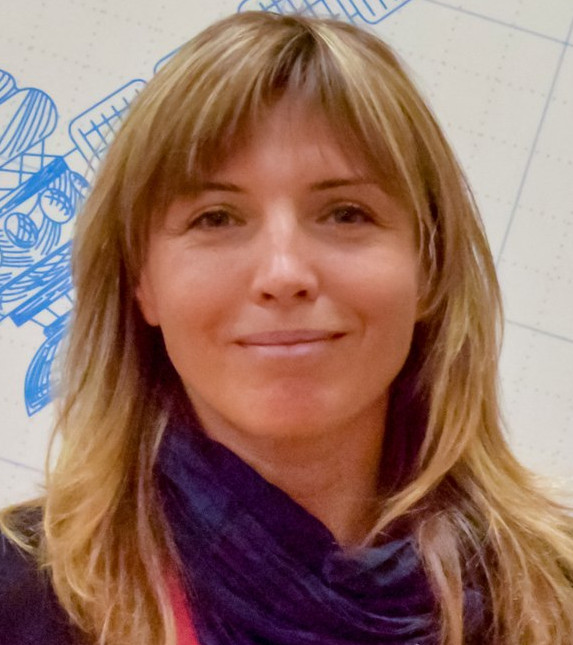
\includegraphics[width=0.75\linewidth]{resources/gorin.jpg}
        \caption{Горина Елена Владимировна \\ \textbf{Зам. дир. по
        фин.-адм. работе}}
    \end{subfigure}
    \begin{subfigure}[b]{0.32\linewidth}
        \centering
        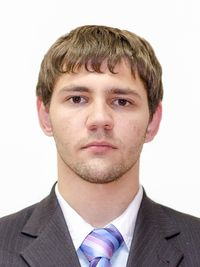
\includegraphics[width=0.75\linewidth]{resources/lvovich.jpeg}
        \caption{Львович Яков Ильич \\ \textbf{Зам. дир. по уч.-восп. работе}}
    \end{subfigure}
    \begin{subfigure}[b]{0.32\linewidth}
        \centering
        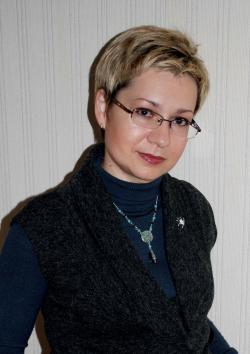
\includegraphics[width=0.75\linewidth]{resources/trofim.jpg}
        \caption{Трофимова Оксана Николаевна \\ \textbf{Старший диспетчер}}
    \end{subfigure}
    \caption{Деканат ФРТК находится в 306 АК. Телефон: +7 (495) 408-54-90, E-mail: dean@frtk.ru}
\end{figure}
%%%%%%%%%%%%%%%%%%%%%%%%%%%%%%%%%%%%%%%%%%%%%%%%%%%%%%%%%%%%%%
\clearpage
\subsection{Управляющие общежитием}
\begin{figure}[h!]
\captionsetup[subfigure]{labelformat=empty,justification=centering,textfont=normalfont}
\captionsetup{labelformat=empty,justification=centering,textfont=normalfont}
    \begin{subfigure}[b]{0.5\linewidth}
        \centering
        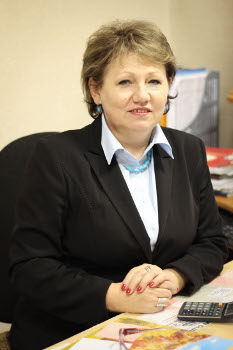
\includegraphics[width=0.75\linewidth]{resources/kazak.jpg}
        \caption{Казакова Ольга Владимировна \\ Телефон: +7 (495) 408-72-39\\ \textbf{Заведующая общежитием №1}}
    \end{subfigure}
    \begin{subfigure}[b]{0.5\linewidth}
        \centering
        
\includegraphics[width=0.75\linewidth]{resources/cvik.jpg}
        \caption{Цвикалова Алёна Петровна \\ \textbf{Кастелянная общежития №1}}
    \end{subfigure}
    \caption{Часы работы: 9:00 — 17:00 (перерыв с 12:00 до 13:00). \\Их кабинеты находятся на первом этаже общежития №1.}
\end{figure}
%%%%%%%%%%%%%%%%%%%%%%%%%%%%%%%%%%%%%%%%%%%%%%%%%%%%%%%%%%%%%%
\clearpage
\subsection{Контакты членов Студсовета}
{
\small
Здесь приведены контакты членов Студсовета,
к которым вы можете обращаться по любым беспокоящим вас
вопросам. Если вы сильно переживаете из-за учёбы, здоровья
или прочих личных вопросов, не стесняйтесь обращаться за
советом к этим ребятам -- они вас обязательно поддержат!
}
\begin{center}
\small
\renewcommand{\arraystretch}{1.1}
\begin{tabular}{ |c|l|c| }
\hline
\textbf{Должность} & \textbf{Имя} & \textbf{Телефон} \\ \hline
Начальник курса & Мурлатов Станислав & +7 (999) 820-06-51 \\ \hline
\multirow{3}{*}{Старшие кураторы}
& Пыталев Максим & $+$7 (917) 125-78-87 \\ \cline{2-3}
& Маслов Роман & $+$ (999) 860-15-15 \\ \cline{2-3}
& Недостоев Кирилл & $+$7 (915) 030-96-11 \\ \hline \hline
\multirow{2}{*}{Кураторы 811 группы}
& Евтушенко Евгений & $+$7 (909) 095-85-95 \\ \cline{2-3}
& Узянов Евгений & $+$7 (910) 228-46-58 \\ \hline
\multirow{2}{*}{Кураторы 812 группы}
& Маршинин Арсений & $+$7 (915) 272-50-64 \\ \cline{2-3}
& Беда Диана & $+$7 (961) 106-27-87 \\ \hline
\multirow{2}{*}{Кураторы 813 группы}
& Тримбач Екатерина & $+$7 (977) 947-92-52 \\ \cline{2-3}
& Кельмяшкин Егор & $+$7 (910) 331-02-70 \\ \hline
\multirow{2}{*}{Кураторы 814 группы}
& Унтилов Ярослав & $+$7 (925) 610-56-08 \\ \cline{2-3}
& Косинов Владислав & $+$7 (953) 107-78-97 \\ \hline
\multirow{2}{*}{Кураторы 815 группы}
& Зудин Дмитрий & $+$7 (953) 436-58-74 \\ \cline{2-3}
& Щербакова Валерия & $+$7 (914) 403-85-58 \\ \hline
\multirow{2}{*}{Кураторы 816 группы}
& Кузнецов Александр & $+$7 (921) 251-05-35 \\ \cline{2-3}
& Просвирин Кирилл & $+$7 (977) 756-33-16 \\ \hline
\multirow{2}{*}{Кураторы 817 группы}
& Колчина Антонина & $+$7 (906) 752-60-76 \\ \cline{2-3}
& Кайдаш Алина & $+$7 (926) 037-20-00 \\ \hline
\multirow{2}{*}{Кураторы 818 группы}
& Зуев Егор & $+$7 (909) 161-61-97 \\ \cline{2-3}
& Дмитриева Марина & $+$7 (915) 207-02-17 \\ \hline
\multirow{2}{*}{Кураторы 819 группы}
& Маркин Иван & $+$7 (916) 417-52-45 \\ \cline{2-3}
& Ягодаров Дмитрий & $+$7 (925) 891-02-23 \\ \hline \hline
Поселяющий ФРТК &&\\ в Долгопрудном & Лаврентьев Кирилл & +7 (977) 834-39-31 \\ \hline
Зам. председателя &&\\ Студсовета ФРТК & Унтилов Ярослав & +7 (925) 610-56-08 \\ \hline
Председатель Студсовета ФРТК & Микоян Филипп & +7 (926) 664-51-59 \\
\hline
\end{tabular}
\renewcommand{\arraystretch}{1}
\end{center}
%%%%%%%%%%%%%%%%%%%%%%%%%%%%%%%%%%%%%%%%%%%%%%%%%%%%%%%%%%%%%%
\clearpage
\section{Часто задаваемые вопросы}
%%%%%%%%%%%%%%%%%%%%%%%%%%%%%%%%%%%%%%%%%%%%%%%%%%%%%%%%%%%%%%
\setcounter{question}{0}
\subsection{Учёба}

\Que{Зачем нужен студенческий билет?}
\Ans{Студенческий билет удостоверяет, что вы являетесь студентом. Также он служит пропуском в учебные корпуса, по нему оформляются все студенческие скидки, и в особых случаях он оставляется под залог. В случае утери в деканате выдается дубликат (при условии денежной компенсации).}


\Que{Какая неделя четная, а какая нечетная?}
\Ans{Первая неделя (3-8 сентября в I семестре и 1-2 февраля во II) является нечетной, далее они чередуются. Какая сейчас неделя, можно узнать на стенде с расписанием.}

\Que{Где узнать расписание?}
\Ans{Расписание висит на первом этаже ГК и на сайте МФТИ \href{https://mipt.ru/about/departments/uchebniy/schedule/study/}{в разделе «Расписание»}. Также ссылка на расписание находится в \href{https://vk.com/page-17708_53431659}{меню сообщества ФРТК МФТИ}, и, кроме того, оно, по мере появления, публикуется в сообществе «Студентов 1-го курса».}

\Que{Как узнать, где находится аудитория?}
\Partans{Список сокращений корпусов:}
\begin{itemize}
    \item АК — Аудиторный Корпус.
    \item ГК — Главный Корпус.
    \item КПМ — Корпус Прикладной Математики.
    \item ЛК — Лабораторный Корпус.
    \item НК — Новый Корпус(редко -- Корпус Микроэлектроники). Также НК означает площадь перед Новым Корпусом.
    \item РТ — Радиотехнический Корпус.
    \item БФК – БиоФармКластер.
    \item Например, 418 ГК — аудитория на 4-м этаже Главного Корпуса, 806 КПМ — восьмой этаж Корпуса Прикладной Математики.
\end{itemize}
\end{minipage}

\Que{Какие существуют сокращения названий аудиторий?}
\begin{itemize}
    \item Гл. Физ. — Главная Физическая аудитория. Находится на 5-м этаже ГК в левой части здания, в самом конце коридора.
    \item Б. Хим./Б. Физ. — Большая Химическая/Физическая аудитория. Обе расположены на 5-м этаже ЛК (Химическая — слева, Физическая — справа).
    \item Акт. Зал — Актовый зал находится на 2-м этаже ЛК по центру.
    \item Лабораторные работы по механике проходят на 5-м этаже ГК, по общей химии — на 4-м этаже ЛК, по термодинамике — на 3-м этаже ГК. Все корпуса, кроме АК, РТ и БФК, соединены переходами.
\end{itemize}
\end{minipage}

\Que{Какие цвета что обозначают в расписании?}
\Ans{Красный — лекции. Синий — семинары. Зелёный -- окна. Желтый — \sout{тоже окна, но другого цвета} лабораторные работы, иностранный язык и физкультура.}

\Que{Где находится библиотека?}
\Ans{Техническая (с учебной литературой) и художественная — на 1-м этаже ГК, библиотека кафедры иностранных языков — 3-й этаж НК.}

\Que{Где получить такую-то справку?}
\Ans{Справка для военкомата получается во втором отделе (330 ГК). Справка о том, что вы являетесь студентом — в учебном отделе (413 АК). Справка о том, что вы живете в общежитии — у кастелянши (1-й этаж общежития № 1).}

\Que{Что такое «задавальник»?}
\Ans{«Задавальник» — это сборник программ и заданий на семестр. В нем содержатся задания по каждому из предметов и календарь их сдачи. Старайтесь не потерять его! Лишний экземпляр найти чрезвычайно сложно. Если же это все-таки случится, еще один экземпляр можно получить (при наличии) в секретариате деканата ФРТК (307 АК) или сделать ксерокопию у однокурсника. Также можно пользоваться электронной версией («задавальники» по соответствующим предметам можно найти на сайтах кафедр).}

\Que{Что такое задание и как его сдавать?}
\Ans{Задание представляет собой набор задач, который нужно решить к определенному сроку, который указан в задавальнике, хотя иногда семинарист может его перенести. Обычно задание оформляется в тонкой (12–24 листов) тетради. Процедура сдачи сильно зависит от преподавателя. Например, семинарист может задать теоретический вопрос, попросить объяснить ему, как вы решали ту или иную задачу, или попросить решить какую-то другую задачу. Настоятельно рекомендуется сдавать задания в срок: это влияет и на отношение к вам преподавателя, и на вашу подготовленность, и на рейтинг по некоторым предметам. Например, полусеместровая контрольная работа по физике проводится на несколько дней раньше, чем сдача первого задания. Таким образом, вам необходимо сделать задание ко дню контрольной работы, чтобы успешно ее написать. Кроме того, на сдачу соответствующего задания может повлиять оценка за коллоквиум по математическому анализу или за контрольную по физике. Получив на них «хорошо» или «отлично» вы либо освобождаетесь от сдачи задания, либо процедура сдачи существенно упрощается (однако, будут ли учтены ваши успехи или нет, зависит от семинариста). К зачетной сессии задания должны быть сданы, иначе вам не поставят зачет (например, по физике или информатике) или вычтут баллы из рейтинга за семестр. Списывать задания не следует, потому что только самостоятельное решение поможет вам наработать необходимые навыки.}

\Que{Какая шкала оценки знаний используется?}
\Partans{С 2010 года в МФТИ параллельно с традиционной пятибалльной системой оценок используется 10-балльная шкала:}
\begin{center}
\begin{tabular}{ |c|c| }
\hline
    \textbf{Оценка по 10-балльной шкале} & \textbf{Оценка по 5-балльной шкале} \\ \hline
    8-10 & «отлично» \\ \hline
    5-7 & «хорошо» \\ \hline
    3-4 & «удовлетворительно» \\ \hline
    1-2 & «неудовлетворительно» \\
\hline
\end{tabular}
\end{center}
\end{minipage}

\Que{Что такое рейтинг (БРС) и по каким предметам он есть?}
\Partans{БРС — балльно-рейтинговая система, использующаяся с целью учета работы студента в семестре при выставлении итоговой оценки по предмету. В рейтинг студента может входить (в зависимости от предмета) посещения занятий, результаты промежуточных контрольных работ и оценки за задания. БРС применяется на кафедрах высшей математики и иностранных языков (а также некоторых других). На кафедре теоретической механики за несданные задания вводится наказание в изощрённой форме. \\ \\ С 2016 года на кафедре общей физики введена поправка к правилам промежуточной аттестации, учитывающая результаты сдачи заданий в течение семестра. К оценке за письменный экзамен, оцениваемый по 10-балльной шкале, прибавляются баллы за сдачу каждого из двух заданий(см.таблицу), при этом оценка за письменный экзамен не может превышать 10 баллов, а оценка за устный экзамен (которая идёт в зачётку), в свою очередь, ограничена сверху оценкой за письменную работу.}

\begin{center}
\begin{tabular}{ |c|c| }
\hline
    \textbf{Прибавка к оценке} & \\
    \textbf{за письменный экзамен} & \textbf{Оценка за задание} \\ \hline
    +2 балла & «отлично» \\ \hline
    +1 балл & «хорошо» \\ \hline
    +0 баллов & «удовлетворительно» \\ \hline
    -3 балла & «неудовлетворительно» \\
\hline
\end{tabular}
\end{center}
\end{minipage}

\Que{Что такое «лабник»?}
\Ans{«Лабник» — книга, содержащая описания к лабораторным работам, которые вам предстоит выполнить. Кроме того, этим словом часто называют преподавателя, ведущего лабораторные занятия.}

\Que{Что такое лабораторный маршрут?}
\Ans{Лабораторный маршрут — порядок выполнения лабораторных работ в семестре. Маршруты по механике можно посмотреть на 5-м этаже ГК, по термодинамике — на 3-м, а также \href{https://mipt.ru/education/chair/physics/S_I/lab/}{на сайте кафедры}.}

\Que{Как выполнять «лабы» и как их сдавать?}
\Ans{Выполнение лабораторной работы включает в себя четыре этапа. Первый этап — подготовка. Дома, до лабораторной работы, вы изучаете теоретический материал, касающийся работы, оформляете тетрадь (записываете кратко теорию, расчетные формулы, делаете рисунок установки, заранее расчерчиваете таблицы). Учтите, что некоторые преподаватели задают вопросы по теории прежде чем допустить к работе. Второй этап — непосредственное выполнение работы в лаборатории, где вы проводите эксперимент и записываете результаты. Третий этап — подготовка к сдаче. После выполнения работы вы повторяете теоретический материал и обрабатываете экспериментальные данные. Четвертый этап — сдача, в ходе которой преподаватель проверяет вашу тетрадь и задает вопросы по теории. Итоговая оценка за работу ставится с учетом подготовки, выполнения и качества отчета.}

\Que{Где можно узнать информацию о преподавателях?}
\Ans{Существует сайт \href{http://wikimipt.org}{Викифизтех}, где есть информация о большинстве преподавателей Физтеха с комментариями студентов и других пользователей. Для того, чтобы оставлять комментарии и видеть скрытые (с низким рейтингом) необходимо иметь ящик в домене phystech.edu.}

\Que{Мне не нравится мой семинарист. Что делать?}
\Ans{Во-первых, можно посещать семинары другого преподавателя параллельно со своими. Во-вторых, есть возможность сменить семинариста по предмету. Для этого требуется заявление в свободной форме, написанное на имя заведующего кафедрой, подписанное новым и старым преподавателями. Вероятно, это повлечет за собой изменения в вашем расписании. Менять семинариста без существенных на то причин не рекомендуется. Имейте в виду, что спустя несколько недель после начала семестра кафедры запрещают менять семинариста.}

\Que{Есть ли дополнительные семинары?}
\Ans{Да, проводятся дополнительные семинары по физике, математическому анализу и аналитической геометрии. Большой популярностью пользуются дополнительные семинары по физике, которые ведет \href{http://wikimipt.org/wiki/\%D0\%9E\%D0\%B2\%D1\%87\%D0\%B8\%D0\%BD\%D0\%BA\%D0\%B8\%D0\%BD_\%D0\%92\%D0\%BB\%D0\%B0\%D0\%B4\%D0\%B8\%D0\%BC\%D0\%B8\%D1\%80_\%D0\%90\%D0\%BB\%D0\%B5\%D0\%BA\%D1\%81\%D0\%B0\%D0\%BD\%D0\%B4\%D1\%80\%D0\%BE\%D0\%B2\%D0\%B8\%D1\%87}{Владимир Александрович Овчинкин}, а также семинары по аналитической геометрии \href{http://wikimipt.org/wiki/\%D0\%96\%D0\%B5\%D1\%81\%D1\%82\%D0\%BA\%D0\%BE\%D0\%B2_\%D0\%A1\%D0\%B5\%D1\%80\%D0\%B3\%D0\%B5\%D0\%B9_\%D0\%90\%D0\%BD\%D0\%B4\%D1\%80\%D0\%B5\%D0\%B5\%D0\%B2\%D0\%B8\%D1\%87}{Жесткова Сергея Андреевича}, удостоенного в 2016 году звания «Лучший преподаватель МФТИ». Эти семинары пользуются такой большой популярностью среди студентов, что имеет смысл занимать место заранее. По математическому анализу популярны семинары \href{http://wikimipt.org/wiki/\%D0\%9A\%D0\%BE\%D0\%B6\%D0\%B5\%D0\%B2\%D0\%BD\%D0\%B8\%D0\%BA\%D0\%BE\%D0\%B2_\%D0\%9F\%D0\%B0\%D0\%B2\%D0\%B5\%D0\%BB_\%D0\%90\%D0\%BB\%D0\%B5\%D0\%BA\%D1\%81\%D0\%B0\%D0\%BD\%D0\%B4\%D1\%80\%D0\%BE\%D0\%B2\%D0\%B8\%D1\%87}{Павла Александровича Кожевникова}. Особенность этих семинаров в том, что на них разбираются некоторые задачи из задания и письменных экзаменов, а также в очень хорошем изложении материала. Всем первокурсникам настоятельно рекомендуется их посещать. С расписанием дополнительных семинаров можно ознакомиться на стендах кафедр высшей математики (4-й этаж ГК) и общей физики (5-й этаж ГК). Также информация о дополнительных семинарах регулярно публикуется в группе студентов 1-го курса в \href{https://docs.google.com/spreadsheets/d/1M6Rw4YA6vlkbj5zYJtBc4Z5bTZ47kVKb2b7ZFDoi3X8/edit#gid=0}{данной таблице}.}

\Que{Что такое коллоквиум?}
\Ans{Под коллоквиумом подразумевается проводимый в середине первого семестра мини-экзамен. Это мероприятие максимально приближено к устному экзамену в конце семестра. Помимо вашего семинариста, на нем могут присутствовать другие преподаватели. Программа коллоквиума составляет примерно половину программы за семестр. Оценка за коллоквиум ни на что не влияет и в зачетку не идет, она лишь показывает студенту, насколько хорошо им усвоен полусеместровый курс. Однако оценка может влиять на рейтинг. Все первокурсники сдают коллоквиум по математическому анализу. \\ \\ Аналогом коллоквиума на кафедре общей физики является проводимая в середине первого семестра письменная полусеместровая контрольная. Всё написанное для коллоквиума верно также и для неё.}

\Que{Что такое зачетная сессия и какие зачеты мне предстоит сдавать?}
\Ans{Зачетная сессия проходит с середины по конец декабря в осеннем семестре и с середины по конец мая в весеннем семестре. В это время, называемое иногда зачетной неделей, каждый студент должен сдать зачет по каждому предмету, по которому нет экзамена или по которому есть лабораторные работы. В первой семестре есть зачёты по истории, общей физике, английскому языку, информатике и физической культуре. Зачет бывает дифференцированный (с оценкой) и недифференцированный (зачет/незачет). В случае отсутствия хотя бы одного зачета (хоть по физкультуре, хоть по английскому — это не важно), студент не допускается до экзаменов. Можно начать получать зачеты еще до начала зачетной сессии, но это зависит от преподавателя по предмету и его требований. Например, оценка по зачету по физике формируется на основе оценок за лабораторные работы, за сдачу заданий и за семестровую контрольную работу. \\ \\ Зачёты также можно получать за доп. курсы, как-то: те студенты, чьим семинаристом по дискретному анализу является Бурцев Алексей Анатольевич, получают у него дополнительно зачёт по математической кибернетике. Ещё популярным доп.курсом является курс по операционной системе Linux, занятия которого традиционно начинаются в час дня в субботу. Его ведёт Штейнберг Мирон Натанович. Редакционная команда памятки рекомендует посещать их студентам, интересующимся программированием.}

\Que{Как проходят экзамены?}
\Ans{Экзаменационная сессия проходит с конца декабря по конец января в осеннем семестре и с начала по конец июня в весеннем. Экзамены существуют письменные и устные. В первом семестре всего 6 экзаменов: письменный и устный по математическому анализу и физике, устный по аналитической геометрии и дискретному анализу. \\ \\ Большинство устных экзаменов проходит так: в назначенное время студенты по группам заходят в аудиторию, где сдается экзамен, сдают зачетку дежурному преподавателю, узнают результаты письменного экзамена (если таковой проводился), тянут билет и начинают готовиться (подготовка составляет от сорока минут до часа). По истечении времени, отведенного на подготовку, свободные преподаватели начинают вызывать студентов для ответа. Сдавать своему семинаристу нельзя, но можно изъявить желание сдавать лектору. В случае получения неудовлетворительной оценки студент должен будет пересдать экзамен. Сроки пересдач определяются за несколько недель до начала сессии. \\ \\ Перед экзаменами проводятся консультации, которые рекомендуется посещать. На консультации перед устными экзаменами стоит приходить, уже выучив бо́льшую часть материала, чтобы задать лектору вопросы по непонятным или неосвещенным в литературе или лекциях местам курса. Именно поэтому советуем вам начать готовиться к экзаменам как можно раньше. Многие консультации (особенно к письменным экзаменам) проводятся в режиме онлайн.}

\Que{Что такое «досрок»?}
\Ans{Досрочная сдача экзамена. Досрочно можно сдавать предметы, по которым нет письменного экзамена. Для допуска к «досроку» необходимо иметь все зачеты и подписанное в деканате заявление. В случае неудачной досрочной сдачи, студент отправляется на пересдачу. Время проведения досрочных экзаменов устанавливает лектор по соглашению с кафедрой. На первом курсе досрочно сдавать можно аналитическую геометрию и линейную алгебру.}

\Que{Зачем нужны «курсы по выбору»?}
\Ans{Каждый студент до конца бакалавриата (т.е. до 4-го курса включительно) может самостоятельно выбирать и сдавать семестровые и годовые гуманитарные курсы по выбору. Также институт предоставляет большое число технических курсов по выбору. Информацию о них можно найти на стенде у расписания в ГК (1-й этаж), а также на досках объявлений. Кроме того, в качестве технического курса по выбору может быть зачтен любой институтский или факультетский курс, которого нет в вашем расписании, но по которому вы получили оценку. Кроме желания развить себя стимулом пройти курс по выбору может быть поднятие среднего балла зачётки, например, с целью повысить свои шансы на получение повышенных стипендий, ведь сдать (особенно, гуманитарный) курс по выбору на хорошую и отличную оценку гораздо проще, чем технический обязательный курс.}

\Que{Можно ли не ходить на физкультуру?}
\Partans{Зачёт по физкультуре ставится за посещение, а также (со второго курса) за сдачу нормативов на специализированных секциях. На диаграмме подробно описаны способы получить зачёт на первом курсе. Информацию о проводимых соревнованиях можно получить в \href{https://vk.com/miptsport}{сообществе «Спортивный клуб МФТИ»}. Также обратите внимание, что «пересдача зачёта», называемая также «теоретический зачёт», возможна только в случае, если большая часть занятий пропущена по уважительной причине. \\ \\  Отсутствие зачета по физкультуре означает также лишение стипендии. Кроме того, при наличии четырёх пересдач/незачётов, студент отчисляется. Незачёт по физкультуре у таких студентов обычно получается первым. }
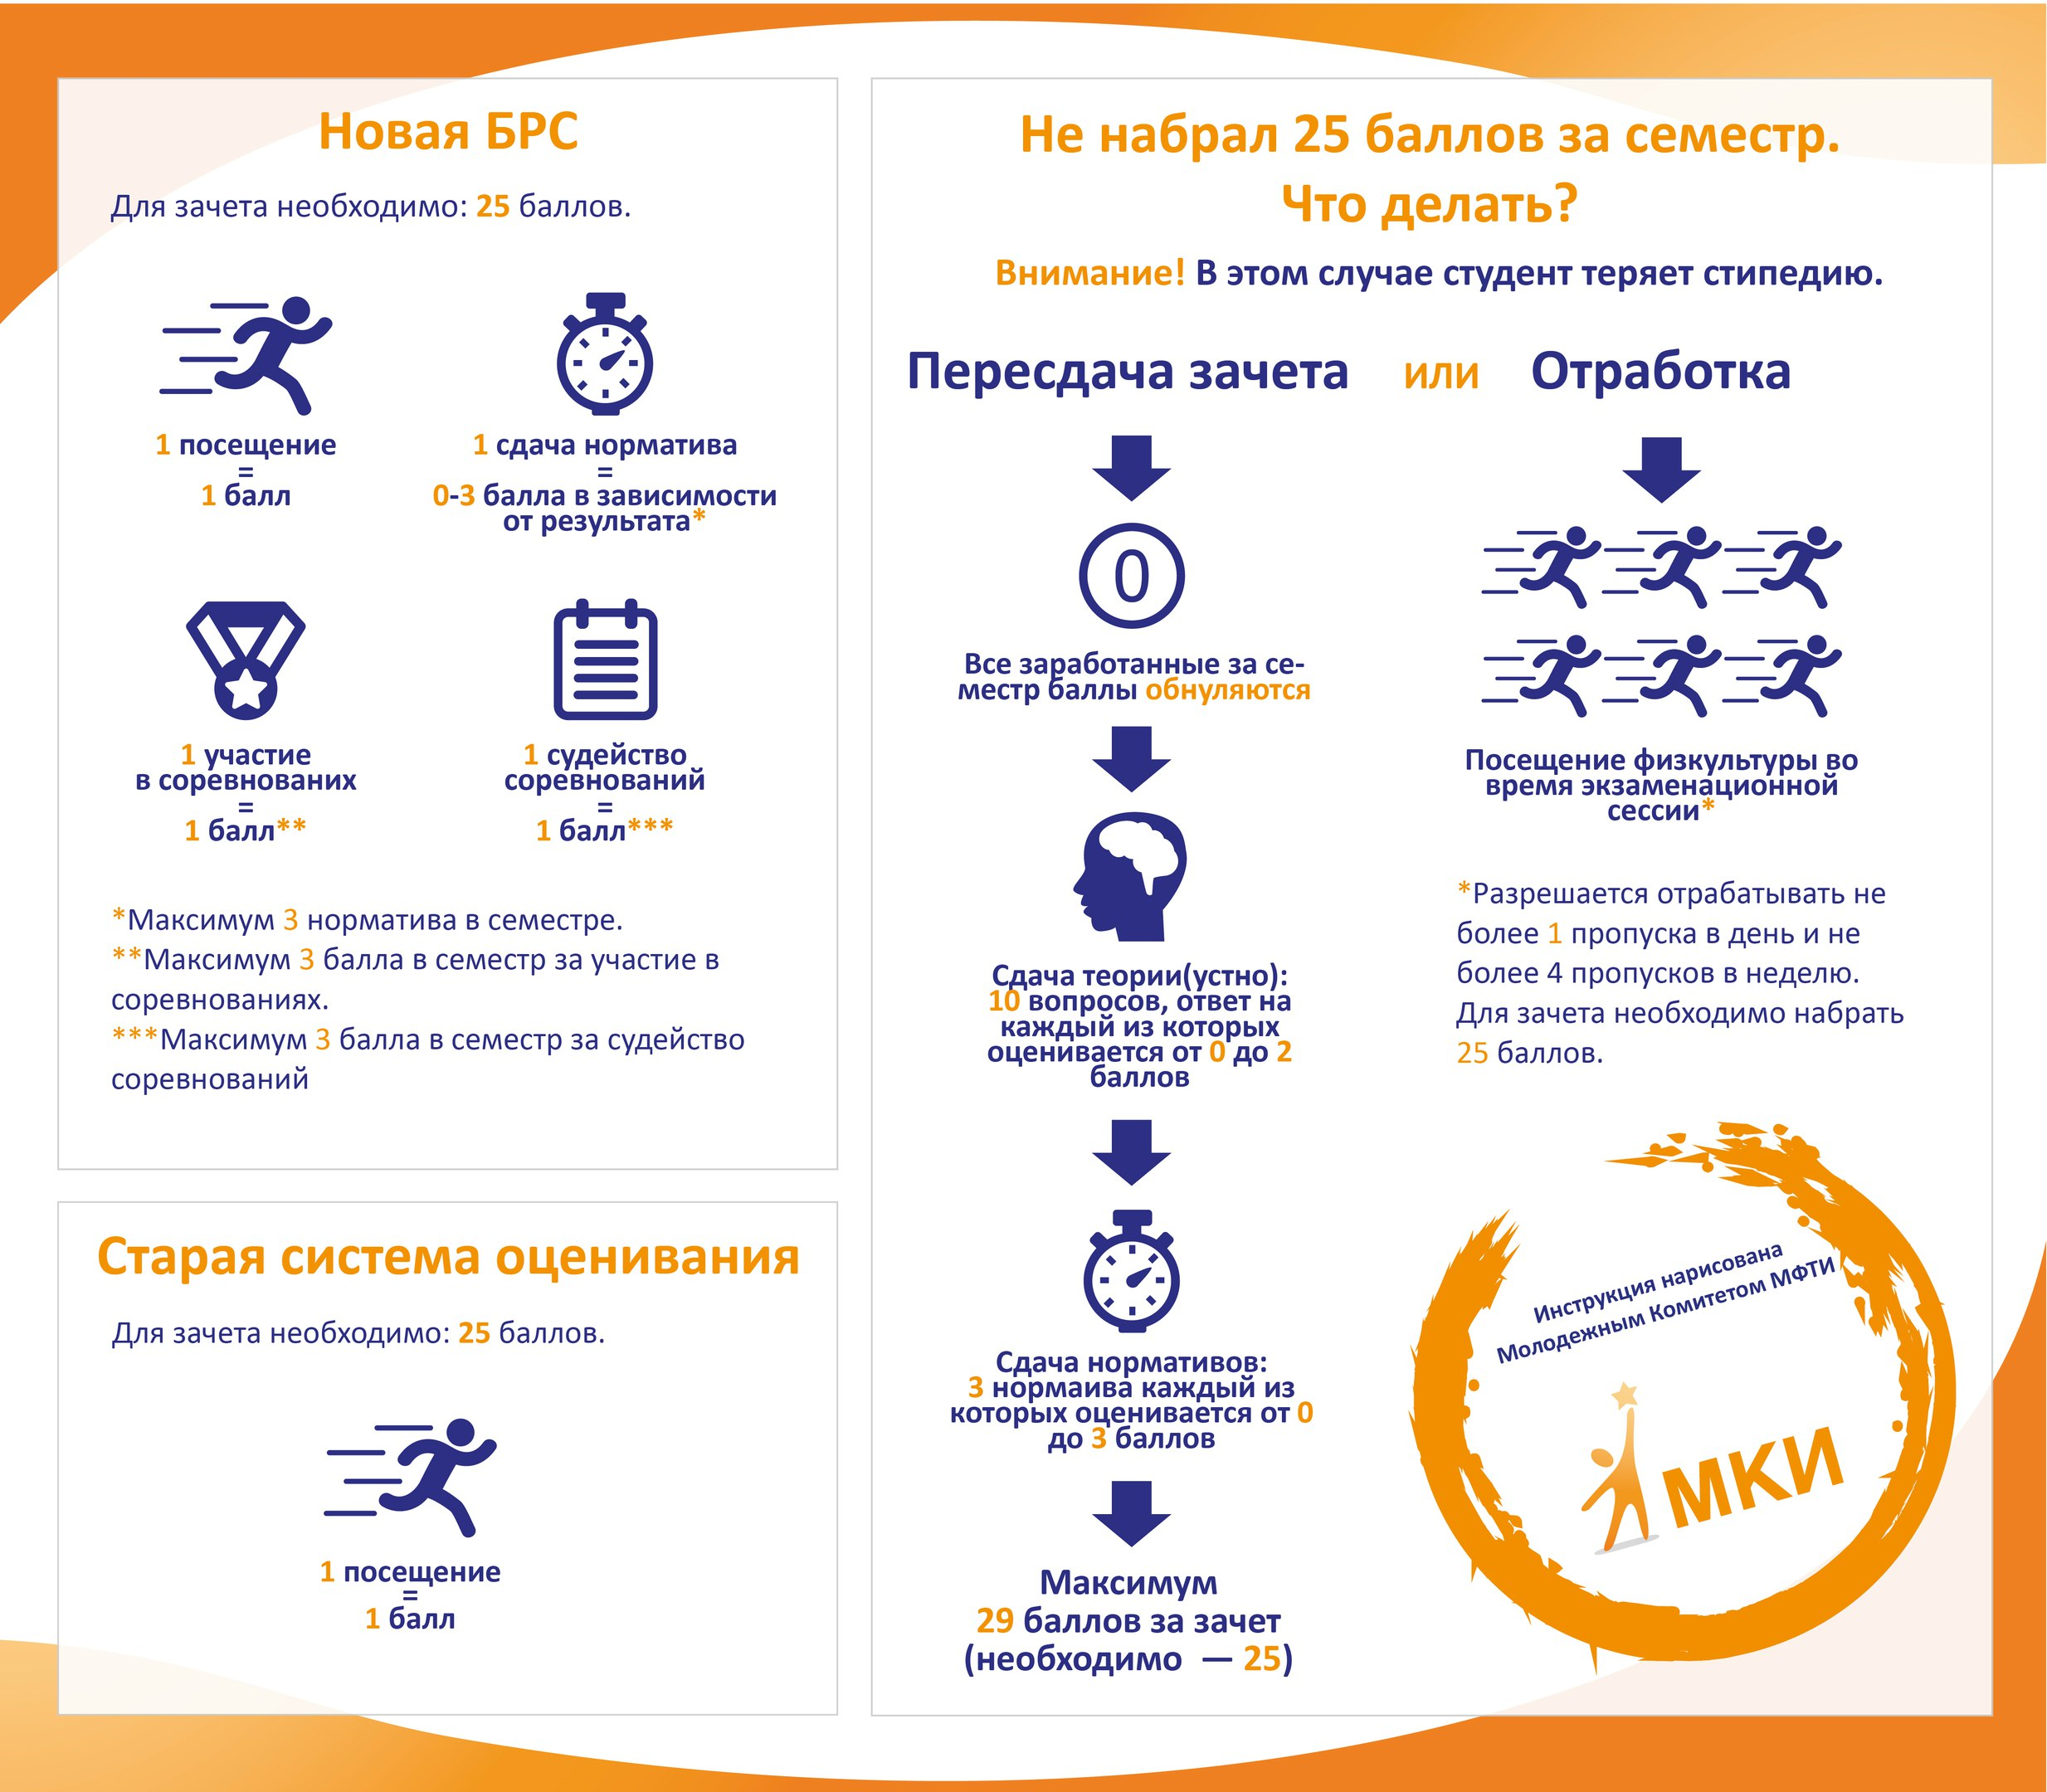
\includegraphics[width = 150 mm]{resources/fizra.jpg}
\end{minipage}

\Que{Я не ходил в школе на физкультуру, что мне здесь делать?}
\Ans{Если у вас проблемы со здоровьем, не допускающие повышенных нагрузок, то стоит сходить в поликлинику и попросить врача (если вы не сделали этого на медосмотре) записать вас в специальную медицинскую группу (СМГ).}

\Que{Какие есть специализации по физкультуре?}
\Ans{Футбол, баскетбол, плавание, легкая атлетика, лыжи, общая физическая подготовка (ОФП) и СМГ. Можно договориться с преподавателем, ведущим вашу специализацию, и ходить на физкультуру в то время, когда вам удобно, а не по расписанию, но не меньше двух раз в неделю. Первое занятие по физкультуре — вводное, на нем расскажут про секции и специализации.}

\Que{Можно ли пропускать занятия?}
\Ans{Пропускать какие-либо занятия категорически не рекомендуется (особенно в первом семестре). Однако большинство лекторов посещение лекций не отмечает. Физкультуру пропускать нельзя, так как оценка по этому предмету ставится за посещение. Посещение занятий по иностранному языку, а также по математическим дисциплинам напрямую влияет на оценку в связи с тем, что кафедрами используется балльно-рейтинговая система. Ни в коем случае нельзя пропускать лабораторные работы, так как каждую неделю вы либо делаете лабораторную работу, либо сдаете ее. В случае пропуска сделать ее в другое время очень сложно.}

\Que{Где находится читальный зал?}
\Ans{В общежитии № 1 есть собственный читальный зал, расположенный на первом этаже возле комнаты охраны. Главный читальный зал МФТИ находится на 2-м этаже ГК, он оборудован интернетом (посредством Wi-Fi) и работает (c 2018 года) с 06:00 до 23:00.}

\Que{Где найти дополнительную литературу?}
\Ans{Дополнительную литературу можно взять в технической библиотеке на 1-м этаже ГК, в локальной сети института, а также на \href{http://lib.mipt.ru}{сайте}. Узнать, какие книги числятся за тобой в бибилиотеке, а также ознакомиться со каталогом доступной художественной литературы можно на \href{http://ruslanlib.phystech.edu/}{данном сайте}. Логином является номер твоего студенческого билета или зачетной книжки, сначала дополненный нулями до 12 знаков (например, для номера 43251 логин 000000043251), а пароль — просто номер (43251). \\ \\ Также есть возможность приобрести учебники в магазине «Физтех.Книга» на 1-м этаже НК.}

\Que{Где можно купить канцтовары?}
\Ans{Ближайший магазин с канцтоварами находится на 1-м этаже НК справа от входа(«Физтех.Книга»). Кроме того, есть киоск на первом этаже в здании Комбината Студенческого Питания(КСП).}

\Que{Как не сойти с ума от учебы?}
\Ans{Занимайтесь спортом, ходите на концерты, старайтесь в выходные выбираться в Москву, стремитесь разнообразить свою деятельность (хобби), вступите, наконец, в Совет студентов! День недели, в который проходят собрания, будет опубликован в начале сентября в группе ФРТК МФТИ. Также обязательно посетите мероприятие «День энтузиаста», на котором будут представлены различные клубы, секции и кружки, которые существуют на Физтехе (например, клуб дебатов, клуб исторического моделирования и другие). Список клубов, которые нам удалось отыскать(со ссылками на сообщества), можно найти \href{https://vk.com/page-17708_53470574}{здесь}. \\ \\ Если у вас есть единомышленники и вы хотите организовать тематическую встречу, или, например, устроить небольшой концерт, непременно найдите свободный день в расписании \href{https://calendar.google.com/calendar/embed?src=ffse5gki3k4f9j266789sbj5ns@group.calendar.google.com&ctz=Europe/Moscow}{клуба общежития №1} или \href{https://frtk.mipt.ru/services/meeting/}{Комнаты для Собраний}, которые обустраивались специально для этого! Также в клубе можно отметить День рождения или любой другой праздник. Для бронирования клуба пишите \href{https://vk.com/denproc}{Денису Прокопенко}, КДС -- \href{https://vk.com/domrachev_alexey}{Алексею Домрачеву}. Клуб начинает свою работу 15 сентября.}

%%%%%%%%%%%%%%%%%%%%%%%%%%%%%%%%%%%%%%%%%%%%%%%%%%%%%%%%%%%%%%
%%%%%%%%%%%%%%%%%%%%%%%%%%%%%%%%%%%%%%%%%%%%%%%%%%%%%%%%%%%%%%

\clearpage
\setcounter{question}{0}
\subsection{Быт}
\subsubsection{Общежитие}

\Que{Какой адрес у общежития № 1?}
\Ans{141701, Московская область, г. Долгопрудный ул. Первомайская, 34/5}

\Que{Как в общежитие приходит почта?}
\Ans{Все извещения о посылках и письма приходят в первое общежитие. Посылки студентам нужно забирать в отделении Почты России, расположенном по адресу ул. Циолковского 4.}

\Que{Я хочу организовать тематическую встречу/небольшой концерт/отметить день рождения и т.п.}
\Ans{В общежитии №1 специально для этого благоустроены клуб(1 этаж) и Комната Для Собраний(КДС, № 214). Клуб больше подходит для концертов и дней рождения, а КДС -- для просмотра фильма в узком кругу друзей или подготовки к экзамену в Технотрек(с компьютерами, маркерная доска расположена в читальном зале на 1 этаже). В первую очередь проверьте, свободен ли интересующий вас день в расписании \href{https://calendar.google.com/calendar/embed?src=ffse5gki3k4f9j266789sbj5ns@group.calendar.google.com&ctz=Europe/Moscow}{клуба} или \href{https://frtk.mipt.ru/services/meeting/}{КДС}(лучше дополнительно уточнить у ответственного). В случае, если день свободен, помещение можно забронировать у ответственного. Ответственный за клуб \href{https://vk.com/denproc}{Денис Прокопенко}, за КДС -- \href{https://vk.com/domrachev_alexey}{Алексею Домрачеву}. Клуб начинает свою работу 15 сентября.}

\Que{Я забронировал клуб на нужную мне дату, но ещё я хотел бы, чтобы всё общежитие узнало о предстоящем мероприятии}
\Ans{Вам следует написать сообщение \href{https://vk.com/danya_goes_ahead}{руководителю Информационного департамента} Совета студентов(его состав можно на сайте ФРТК в разделе \href{https://mipt.ru/drec/forstudents/studsovet/structure.php}{«Структура Совета студентов ФРТК»}), чтобы он решил, в какие сообщества и в каком формате следует опубликовать новость. Кто знает, может ваше мероприятие получит такой отклик, что в следующий раз дизайнеры Информационного департамента подготовят афишу, а Совет студентов поможет вам с закупкой еды участникам? Если вы действительно горите желанием работать во благо студентов, непременно свяжитесь с \href{https://vk.com/philalala}{председателем Студсовета}, вам помогут найти себя в мире активизма!}

\Que{Какой распорядок в общежитии?}
\Ans{В общежитии после 23 часов должна быть тишина в соответствии с законом РФ «О тишине» (ФЗ № 52). Не мешайте людям спать, особенно своим соседям. Если в общежитии устраиваются шумные вечеринки в коридорах, то это наказывается мерами вплоть до выселения и исключения из института. Если вам мешает шум в позднее время, то в первую очередь не стесняйтесь сообщить об этом шумящим. Если после этого шум продолжится, то рекомендуем обращаться к ответственным по этажу (их контакты есть на стендах в общежитии и на сайте факультета) или к другим представителям Студсовета. В самом крайнем случае можно обратиться к охраннику общежития. \\ \\ Войти в своё общежитие, имея на руках пропуск, можно в любое время. В остальные общежития можно попасть до часа ночи. Не надо пытаться вылезти или залезть в общежитие нетрадиционным образом (то есть не через дверь), так как это заканчивается обычно переломами и выговорами.}

\Que{Можно ли готовить в комнате на электроплитке?}
\Ans{Нельзя. Это является грубым нарушением правил пожарной безопасности. Комендант общежития и студенческая комиссия вправе изъять электроплитку до окончания разбирательства, которое может закончиться выселением и отчислением.}

\Que{Где можно поесть?}
\Ans{Поскольку в общежитии № 1 буфет отсутствует, студенты либо сами готовят себе еду, либо питаются в столовых. Общеинститутская столовая «Комбинат Студенческого Питания» находится в здании через дорогу от общежития № 1. Также столовые есть на 2-м этаже ГК, НК и КПМ. Столовые \href{http://veryfood.ru}{в КПМ} и \href{http://3ka-food.ru/}{в третьем общежитии} доставляют еду по кампусу. Неплохая подборка заведений, где можно поесть студентам Физтеха, расположена на сайте \href{http://foodmipt.ru/}{foodmipt.ru}.}

\Que{Как работает душ?}
\Ans{Душ работает круглосуточно 7 дней в неделю.}

\Que{Как пользоваться стиралкой?}
\Ans{Авторизироваться \href{https://frtk.mipt.ru}{на сайте Студсовета ФРТК} и следователь инструкциям, указанным там.}

\Que{Можно ли заводить в комнатах животных?}
\Ans{Формально, согласно новым положениям об общежитиях, нельзя. Но поскольку строгость законов компенсируется необязательностью их исполнения, почти в каждом общежитии живут «свои» кошки и коты. В общежитии №1 это Полторашка. И хотя мы не рекомендуем заводить домашних животных хотя бы потому, что того требует устав института, вы можете попробовать. Но имейте в виду, что если ваше животное будет как-то мешать соседям(по комнате, коридору или общежитию) звуками, запахами или как-то иначе, у вас имеют право потребовать удалить животное из общежития. \\ Тараканы, крысы (за исключением купленных в зоомагазине) и клопы к домашним животным не относятся и подлежат уничтожению (см. следующий пункт).}

\Que{Что делать, если в моей комнате завелись тараканы, клопы или мыши?}
\Ans{Нужно сообщить об этом кастелянше и записаться в список на санитарную обработку комнаты.}

\Que{Есть ли в общежитии общественные пылесос/аптечка/сканер/противень для духовки?}
\Ans{Да, есть. Смотри также список предметов общего пользования на сайте ФРТК. Все эти предметы выдаются студентам и аспирантам ФРТК, проживающим в общежитии № 1 под залог студенческого билета. Информацию о том, у кого их можно взять, можно найти на сайте ФРТК в разделе \href{https://mipt.ru/drec/forstudents/studsovet/structure.php}{«Структура Совета студентов ФРТК»}, либо в закреплённой записи \href{https://vk.com/frtk_dorm}{группы общежития}.}

\Que{Как пользоваться общественным принтером в общежитии?}
\Ans{Для этого надо завести аккаунт на сайте \href{http://print.mipt.ru}{print.mipt.ru} или \href{https://printbox.io/}{printbox.io}(эти сервисы конкурируют) и следовать инструкциям. Принтеры есть в каждом общежитии.}

\Que{Ко мне приезжают родственники. Можно ли их оставить на ночь в общежитии?}
\Ans{Да, возможно размещение родственников или друзей в общежитии. Для этого необходимо заранее обратиться к коменданту общежития. В случае неожиданного приезда гостей в выходные или праздничные дни, нужно обратиться к охраннику общежития с просьбой разместить их в гостевой комнате до прихода коменданта.}

\Que{У меня в комнате не работает розетка/разбито стекло/сломалась полка. Что делать? / В умывалке третий день течет кран! Кому об этом сказать?}

\Partans{Сообщить о любой неисправности в общежитии можно тремя различными способами:}
\begin{itemize}
    \item сообщить о проблеме в группе ВКонтакте «Общежитие ФРТК»
    \item записать неисправность в журнал у охранника
    \item сказать об этом коменданту
\end{itemize}
\end{minipage}

\Que{Можно ли жить в другом общежитии или хотя бы поменяться комнатами?}
\Ans{Можно. Для этого должны быть согласны соседи всех комнат, а также поставлен в известность комендант общежития, где вы хотите жить. В случае переселения по обмену, нужно написать соответствующее заявление (образец есть на сайте ФРТК), подписать его у комендантов обоих общежитий, а также у директора студгородка.}

\subsubsection{Спорт и здоровье}

\Que{Что делать, если я заболел?}
\Ans{Немедленно идти к врачу в поликлинику МФТИ (она находится в здании санатория-профилактория между общежитиями № 4 и № 6). Для экстренных ситуаций на 1-м этаже поликлиники МФТИ работает травмпункт. Также в любой момент можно попросить охранника общежития вызвать «Скорую помощь». Для прохождения некоторых видов обследования (например, флюорографии) или для консультации с профильным специалистом может потребоваться посещение больницы г. Долгопрудный, которая находится в конце улицы Первомайская (высокое белое здание).}

\Que{Есть ли межвузовские спортивные соревнования?}
\Ans{Конечно, есть. Если вы себя хорошо проявите, занимаясь тем или иным видом спорта, то вы сможете попасть в сборную института. Обращайтесь по этому вопросу к преподавателям секций физкультуры. Подсказка: участие в межфакультетских и межвузовских соревнованиях даёт бонус при переселении в общежития квартирного типа.}

\Que{В чем разница между специализацией и секцией?}
\Ans{Специализация — тот вид спорта, которым вы будете заниматься на занятиях физкультурой. Помимо этого, вы можете ходить в секцию по какому-то виду спорта, куда, однако, берут тех, кто имеет подтверждение своих успехов и заслуг (разряд, грамоты с соревнований). В отдельных случаях преподаватель, ведущий секцию по виду спорта, который не существует как специализация (например, настольный теннис) может выставлять вам зачет по физкультуре.}

\Que{Что такое санаторий-профилакторий, как туда попасть? }
\Ans{Профилакторий — это то место, где можно восстановить здоровье, проживая в комнате с меньшим числом соседей и проходя лечебные процедуры. Проживающие в профилактории обеспечиваются трехразовым питанием, витаминами и при необходимости лекарствами. В профилактории менее шумно, чем в общежитии, там можно выспаться, отдохнуть от соседей и спокойно позаниматься. Информация о том, как можно получить путёвку в санаторий-профилакторий, регулярно публикуется в сообществе Профкома студентов. Поселиться в профилакторий можно один раз в семестр.}

\Que{Как пользоваться спортивной комнатой общежития?}
\Ans{Ключ от спортивной комнаты («качалки») выдается под залог студенческого билета ответственными членами Студсовета. Номера комнат, в которых выдается ключ, написаны на двери в спортивную комнату и на сайте ФРТК в разделе «Структура Совета студентов ФРТК». Охранник ключ от качалки не выдает!}

\Que{Я не попал на специализацию плавания. Могу ли я все-таки ходить в бассейн?}
\Ans{Да, есть сеансы оздоровительного плавания. Расписание можно узнать на втором этаже здания Бассейна. Для посещения сеансов необходимо взять справку в поликлинике МФТИ у терапевта ФРТК. Расписания работы врачей в поликлинике МФТИ регулярно публикуются в сообществе \href{https://vk.com/students_of_mipt}{Физтех.Сегодня}.}

\subsubsection{Деньги(стипендия и работа)}

\Que{Какую сумму составляет стипендия и какие они бывают?}
\Ans{Государственная академическая стипендия составляла в осеннем семестре 2017-2018 учебного года для победителей всероссийских олимпиад по профильным предметам – 15000 рублей; для победителей и призёров за последние три года, предшествующих году поступления, трёх и более олимпиад РСОШ – 11800 рублей; одной олимпиады РСОШ -- 9500; для остальных студентов первого курса – 6600 рублей. \\ \\ Также существует социальная стипендия. Чтобы ее получить, нужно взять справку в социальном отделе в своем родном городе, которая выдается на основании справок о доходах членов семьи. Иностранные граждане получать социальную стипендию не могут. \\ \\ Стипендия фонда Абрамова-Фролова начисляется студентам с 1-го по 3-й курс и составляет 12000 рублей в месяц. Назначаются на эту стипендию студенты с тяжелым материальным положением и отличники учебы.}

\Que{Как получить материальную помощь?}
\Ans{Чтобы получить матпомощь от деканата, нужно написать заявление, в котором обоснована причина, по которой она вам требуется, и отдать старосте курса (до его назначения заявления собирает начальник курса). Объявления о начале приема заявлений на матпомощь в начале каждого месяца появляются на стендах в общежитии. Также можно раз в семестр получить матпомощь от профсоюза в размере 1200 рублей, для этого нужно прийти в профком, написать заявление и отдать его профоргу факультета. Для этого при заполнении заявления на матпомощь нужно принести с собой чеки на строительные материалы или мебель. {\em \bfВнимание:} платники, а также студенты, находящиеся в академическом отпуске, материальную помощь получать не могут. }

\Que{Можно ли на первом курсе совмещать работу с учебой?}
\Ans{Да, но только если это работа в ЗФТШ, либо это разовая работа. Работать в ЗФТШ достаточно интересно и не слишком трудно. Вам, как преподавателю, нужно будет проверять работы учеников. Платят около 80 рублей за час (две тетради: тетрадь по физике и тетрадь по математике). Всякая другая работа, например, в каких-либо фирмах, характеризуется так: либо учеба, либо работа. Поэтому рекомендуем вам повременить с началом трудовой деятельности.}

\Que{Как оформить Социальную карту студента?}
\Ans{Карты оформляются в МФЦ г. Москвы (в МФЦ Московской области карты не оформляются) по предъявлению студенческого билета и паспорта при наличии ваших данных в реестре студентов. \\ Проверить наличие данных в реестре можно на сайте \href{https://www.mos.ru/socialnaya-karta/services-proverka-grazhdanina-v-reestre-studentov/}{https://www.mos.ru/}. Обычно данные появляются в реестре спустя некоторое время после начала учебного года. \\ Адреса МФЦ можно узнать по ссылке \href{https://pgu.mos.ru/ru/mfc/}{https://pgu.mos.ru/ru/mfc/}. \\ \\ Для начисления стипендии на социальную карту студента необходимо сообщить её номер в социальный деканат(2 этаж КСП).}

\Que{Можно ли начислять стипендию на карточку другого банка?}
\Ans{Да, можно, для этого необходимо с 11.00 до 18.00 в рабочий день подойти с реквизитами карты в социальный деканат(2 этаж КСП) и на месте заполнить заявление о начислении на неё стипендиальных выплат. }

\subsubsection{Компьютер/Интернет}

\Que{Нужен ли на первом курсе собственный компьютер?}
\Ans{Да, его желательно иметь, так как многие задания есть только в электронном виде, на нем удобно рассчитывать результаты лабораторных работ, задания по информатике также удобнее выполнять дома.}

\Que{Как и где подключиться к Интернету?}
\Ans{К Интернету можно подключиться в МФТИ-Телекоме (1-й этаж КПМ, кабинет 109). Студентам, проживающим в студгородке, предоставляются особые тарифы типа «Академический», среди которых есть в том числе и предоставляющие безлимитный доступ в Интернет. С актуальными ценами можно ознакомиться на \href{http://mipt-telecom.ru/}{сайте}.}

\Que{В моей комнате не работает сетевая розетка/нет кабеля. Что мне делать?}
\Ans{Обратиться в МФТИ-телеком. Интернет можно провести по кабелю в комнату, а можно оплатить подключение к интернету через Wi-Fi. Роутеры МФТИ-телеком расположены на каждом этаже первого общежития, а кабели проведены в каждую комнату. Кроме того, дешевизна предоставляемых услуг делает выгодным регистрацию дополнительного аккаунта с оплаченным Wi-Fi подключением для использования интернета в пределах всего кампуса.}

\Que{Как получить электронную почту на доменах frtk.ru или phystech.edu?}
\Ans{Для получения электронной почты на домене frtk.ru, вам следует написать сообщение любому сотруднику Информационного департамента Совета студентов(его состав можно на сайте ФРТК в разделе \href{https://mipt.ru/drec/forstudents/studsovet/structure.php}{«Структура Совета студентов ФРТК»}). Владельцам электронных почтовых ящиков на этом домене предоставляется облачное хранилище неограниченного размера. \\ \\ Для получения электронной почты на домене phystech.edu, которая может пригодиться для бесплатного получения лицензионного ПО и владельцам которой также предоставляется безлимитное облачное хранилище, необходимо отправить запрос по электронной почте на helpdesk@mipt.ru или обратиться в техподдержку через личный кабинет на сайте mipt.ru, предоставив любой документ, связывающий вас с МФТИ (например, студенческий билет, зачетная книжка или диплом).}

\subsubsection{Прочие вопросы}

\Que{Что такое профком?}
\Ans{Профком — это профсоюзный комитет студентов. Вступление в него происходит в массовом порядке в начале учебного года, о чем сообщат заранее. У студентов-бюджетников каждый месяц будет удерживаться 1\% от стипендии в качестве материальных взносов. Студенты платной формы обучения платят за членство в профкоме 600 рублей в год. Являясь членом профсоюза, студент может получить путевку в профилакторий, льготную путевку в летний лагерь, купить со скидкой билеты в театр. Профком находится в 224 аудитории ГК.}

\Que{Как получить отсрочку от армии?}
\Ans{Необходимо взять во втором отделе (330 ГК) справку для военкомата, сделать ксерокопию паспорта и временной регистрации и отнести это все (не забудьте приписное свидетельство) в военкомат г. Химки (для студентов старше 18 лет).}

\Que{Как добраться до военкомата?}
\Ans{Адрес военкомата: Химки, проспект Мира 11. Телефоны: +7 (495) 575-87-96 (дежурная часть), +7 (495) 575-87-86, +7 (495) 575-21-23. \\ \\ Доехать в Химки можно либо на автобусе со станции Долгопрудная или на электричке: сначала от станции Долгопрудная до платформы Окружная, затем пересесть на Ленинградское направление на платформу Петровско-Разумовская и далее до станции Химки.}

\Que{Где находится почтовое отделение?}
\Ans{Ближайшее почтовое отделение находится на улице Циолковского, 4, в задании на углу с Институтским переулком.}

\Que{Какие есть поблизости магазины?}
\Ans{Возле общежития № 3 работает несколько круглосуточных киосков. На пересечении улицы Первомайской и Институтского переулка есть магазин «Ардис». Прямо по улице Первомайской в сторону станции Долгопрудная, находится магазин «Мираторг». На станции «Лианозово» есть гипермаркет «НАШ», на станции Марк — гипермаркет «О’Кей» в ТРЦ «РИО»(сохраняйте бдительность, он уже два раза горел). Стройматериалы можно приобрести в магазине «Свет» в начале улицы Дирижабельной, а на Долгопрудненском рынке (радом со станцией) есть два хозяйственных магазина. За бытовой техникой можно съездить на Савеловский рынок.}

\Que{Где можно сделать ксерокопию?}
\Ans{Отксерокопировать что-либо можно прямо в общежитии, связавшись с \href{https://vk.com/domrachev_alexey}{ответственным за сканер} и распечатав скан на принтере print.mipt или printbox. Также можно попросить сделать ксерокопию в деканате (306 АК). Платная копировальня находится в одном здании с Subway, рядом с бургерной.}

\Que{Где сделать фото на документы?}
\Ans{Идите по улице Первомайской до следующего за «Мираторгом» здания(за парком и памятником скорбящей матери). В торце этого здания находится канцелярский магазин и центр «Срочное фото».}
%%%%%%%%%%%%%%%%%%%%%%%%%%%%%%%%%%%%%%%%%%%%%%%%%%%%%%%%%%%%%%
\clearpage
\section{Расписание работы столовых}
\begin{center}
\begin{tabular}{ |c|c| }
\hline
\textbf{Столовая} & \textbf{График работы} \\ \hline

\multirow{2}{*}{Столовая МФТИ}
& 7:30 — 18:00 \\
& Ежедневно \\ \hline

\multirow{2}{*}{Столовая ГК}
& 9:00 — 17:00 \\
& Выходные: суббота, воскресенье \\ \hline

\multirow{2}{*}{Столовая КПМ}
& 10:00 — 22:00 \\
& Ежедневно \\ \hline

\multirow{2}{*}{Столовая НК}
& 9:00 — 17:00 \\
& Выходные: суббота, воскресенье \\ \hline

\multirow{2}{*}{Буфет 3-ки}
& 9:00 — 23:59 \\
& Ежедневно \\
\hline
\end{tabular}
\end{center}
%%%%%%%%%%%%%%%%%%%%%%%%%%%%%%%%%%%%%%%%%%%%%%%%%%%%%%%%%%%%%%
\clearpage
\section{Источники и полезные ссылки}
\begin{itemize}
    \item \href{https://vk.com/drec_mipt}{Сообщество ФРТК МФТИ}
    \item \href{https://vk.com/drec_81x}{Сообщество 1-го курса ФРТК МФТИ}
    \item \href{https://vk.com/page-17708_53431599}{Подборка полезных ссылок в сообществе ФРТК МФТИ(многие ссылки здесь, мы не дублировали)}
    \item \href{https://mipt.ru/about/general/contacts/phones.php}{Телефонный справочник МФТИ}
    \item \href{http://miptstream.ru/2017/08/22/how_not_to_screw_up_3/}{Статья СМИ Поток «Как приехать на Физтех и не облажаться 2017 года»}
    \item \href{https://mipt.ru/students/1kurs.php}{Справочник первокурсника(МФТИ)}
    \item \href{https://mipt.ru/drec/abitur/faq.php}{FAQ для абитуриентов(ФРТК)}
\end{itemize}
%%%%%%%%%%%%%%%%%%%%%%%%%%%%%%%%%%%%%%%%%%%%%%%%%%%%%%%%%%%%%%

\end{document}
